% 来源：OEBPS/Text/Section0001_split_002.xhtml#sigil_toc_id_22

\BookChapter{13}
\section[第13章\q 投资营销谎言8：“高风险才有高收益”]{第13章\\ 投资营销谎言8：“高风险才有高收益”}

\begin{BookQuote}
投资操作，就是通过深入、完全的分析，保证本金的安全性和足够高的收益率。不能满足这些要求的操作就是投机。

\hfill ——本杰明·格雷厄姆（《聪明的投资者》作者）
\end{BookQuote}

\subsection{来拿你的蛋糕，吃掉它}

\begin{BookQuote}
从表面上看，我觉得这就像一个企业家对风险有很高的容忍度。但是我一生中最重要的一句格言就是“下跌有保护”。

\hfill ——理查德·布兰森（维珍航空的创始人）
\end{BookQuote}

我的朋友理查德·布兰森是维珍航空的创始人，也是很多传奇品牌的创始人。1984年，他决定创立维珍航空公司。他知道这就像“戴维挑战巨人歌利亚”一样，不过这位市场营销大师知道，自己可能会让那些竞争对手干掉，特别是那个规模庞大的竞争对手——英国航空。在局外人看来，这好像是一场巨大的赌博。但是理查德·布兰森，就像很多聪明的投资者那样，更关注的是如何对冲下行风险，而不是打出一个本垒打大赢一把。所以理查德·布兰森采取了一个非常聪明的举动，他第一次购买了5架飞机，但是想方设法地协商出一个永久的交易：如果这家公司没能经营好，他可以把买的5架飞机还回去！这是一个能够拿回本钱的保证！他如果失败了，也没有什么损失，但是他如果赢了，就会赢得很大。后面的事情，大家都知道了，他真的赢了，而且赢得很大。

与企业界不一样，投资界会直接告诉你或者非常委婉地告诉你，你如果想大大地赢一把，就必须承担相当高的风险，或者更严肃地说，你如果想获得财务自由，就必须用你的个人自由去冒险。

\subsection{好像没有什么能更偏离真理了}

所有成功的投资内行都有一个共同的特点，他们不会用自己辛辛苦苦攒的钱去做投机，他们会制定策略。请记住沃伦·巴菲特的两条投资法则：第一条，不要亏钱；第二条，记住第一条。不管是世界上顶尖的对冲基金交易人，如瑞·达利欧和保罗·都铎·琼斯，还是像Salesforce.com网络公司的创始人马克·贝尼奥夫，以及维珍航空的创始人理查德·布兰森，无一例外，所有成为亿万富豪的投资内行都在寻找机会，能够让自己得到风险—收益不对称的机会。这是一种书面的说法，它的意思是你得到的收益很高，但你为此承担的风险很低，二者严重不成比例。

\subsection{风险很小，收益很大}

冒的风险很小，赚到的利润很多。最好的例子就是高频交易员，他们用最新的高科技（是的，甚至是飞行机器人和微波塔，传输速度比光速还快），力争节省1/1000秒。你猜他们的风险—收益比是多少？股票市场70\%的交易量都是由他们创造的。我来给你一个线索。威图金融是全世界最大的高频交易公司，它将要公开发行股票上市。按照上市流程规定，它必须披露其业务模式和赢利能力。在过去五年中，它只有一年亏钱了；在过去一年上千个交易日内，只有一个交易日亏钱了！它的风险是什么？我猜想是用更快的电脑做投资。

\subsection{两个硬币相互摩擦}

我的朋友，也是对冲基金的大师凯尔·巴斯在投资界非常有名。他最大的成就是把3000万美元的投资变成了20亿美元，而且只用了短短两年。按照传统的智慧，人们会说他一定承担了非常大的风险，才能获得600多倍的收益。事实并非如此，凯尔只是做了一个赌博，他赌房地产泡沫将会扩大，就像动画片《欢乐糖果屋》里面的小孩一样，这种泡沫迟早都会爆掉。还记得那些日子吗？那些非常贪婪的、不合格的房地产抵押贷款购房人，受到销售人员的劝诱，什么样的房子都敢买。他们没有足够的现金支付，也没有任何证据证明他们负担得起。银行等贷款人不停地发放抵押贷款，因为他们知道他们可以把这些抵押贷款打包，再卖给那些并不真正了解这些抵押贷款实情的投资人。这个泡沫显而易见，只要你站在外面仔细地观察足够长的时间。但是凯尔的聪明过人之处在于，他只冒了3美分的下行风险，就得到了1美元（100美分）的上行收益。冒这么小的风险，就能得到这么高的潜在收益，他是怎么做到的？

最近我和凯尔交流，他详细地分享了另外一个风险—收益严重不对称的投资机会。这个机会的投资条件是什么？他投资本金的95\%有保证，如果公司公开上市，他就会有无限的上行收益（他预期会得到巨大的回报）。但是如果这家公司股价大跌，甚至公司都跌没了，他的损失最多只有5\%。

凯尔就像所有伟大的投资者一样，承担了很小的风险，却有机会获得很大的回报。用力去击球，想要打出一个本垒打，大赢一把，却没有任何下行风险保护，这是灾难的根源。

“我怎么讲这个观点，读者才能一听就懂？”我问。

“托尼，我来告诉你我是怎样教两个儿子，让他们搞明白的：我们买了5美分硬币。”

“你说什么，凯尔？是不是刚才电话出问题了？我敢发誓，你刚才说的是你买了5美分硬币。”

“你听得很清楚。有一天，我正站着冲澡，忽然想，我怎样才能得到完全没有风险的回报？”

大部分投资专家做梦也不敢想会有这样的好事。在他们的脑子里，无风险收益是一个自相矛盾的说法。像凯尔这样的投资内行跟大众的想法完全不同。他总是故意违反传统智慧，来寻找风险—收益严重不对称的小规模的投资机会。这位著名的风险投资大师创造了最近100年来最高的业绩，却用自己辛辛苦苦挣来的钱去买钱：投资200万美元购买5美分硬币，这些硬币挤满了一间小屋。这是怎么回事？

5美分硬币的价值不断波动，就在我跟凯尔进行电话交流的时候，他告诉我：“托尼，美国一个5美分硬币要是熔成金属（镍），其价值为6.8美分。这意味着5美分硬币其实真正的价值是6.8美分（增值36\%）。”想一想，多么疯狂，多么不可思议！我们生活在这样一个世界上，政府花了接近9美分的总成本（包括原材料和制造成本）来制造一个5美分镍币。美国国会有一个人注意到这件事了吗？很明显，这是不可持续的。总有一天，美国国会会醒悟，美国就会改变5美分硬币制造的“原料”配方。“也许下一代5美分硬币会是由锡或者钢铁做的。政府对1美分硬币做过这种完全相同的事情，因为在20世纪80年代早期铜变得太昂贵了。”1909—1982年，1美分硬币是用95\%的铜做的。现在，1美分硬币大部分成分都是锌，只有2.5\%是铜。现在这些老版的1美分硬币的价值是2美分（不是熔化后的价值，是那些硬币收藏者愿意支付的价格）。和原来的票面价值相比，交易价格涨了100\%。如果那个时候你投资了1美分硬币，你的钱就会翻上一番，且没有任何风险，你甚至根本不用熔掉这些1美分硬币。

我承认这种做法一开始听起来有些像耍小花招，但是凯尔是非常严肃和认真的。“要是我能把所有的个人财富都换成钱拿出来，我就把它们换成5美分硬币，现在我就愿意做这件事。”他解释说，“因为你根本不用担心政府印了多少钱。5美分硬币总是值一个5美分硬币。”他的现金将会升值36\%，就像1美分硬币那样，未来也可能升值100\%，因为美国政府最终不可避免地会改变5美分硬币的配方，使用更便宜的金属。

凯尔非常热心。“我到哪里能够找到这种既能带来36\%的收益率又没有任何风险的投资机会？即使我判断错了，我也会开始有多少钱，将来还能有多少钱。”当然，现在把你的5美分硬币熔掉是不合法的，但是关键是“我并不需要熔掉，因为只要美国政府改变了制造5美分硬币的配方，老版的5美分硬币就会变得比以前更有价值，因为它们具有短缺性了。这些5美分硬币开始从流通领域里退出了，而且越来越短缺了”。

显然，他的孩子们学到了这一课，而且他们的身体也得到了很好的锻炼，因为他的孩子们要把一箱箱硬币搬到他们家的储藏室里。

现在你也许会想：“是的。对于凯尔·巴斯来说这样的投资确实很棒，他有百万美元甚至亿万美元的财富可以做大手笔的投资，但是我的钱很少，如何用这种方式投资？”当然，对于普通投资者来说，根本不可能只有上行收益而没有下行风险，即本金可以得到保护，不会遭受损失，而且有很大的上行收益潜力。

你再好好想想。

同样高水平的金融创新推动了高频交易快速发展，从不存在到发展成为股市主导力量，只用了十年，这也触动了金融界的其他领域。2008年金融危机，股市崩盘之后，很多人并没有意愿投资股票，在全球最大的银行工作的非常有创意的聪明人，想出了一套办法，完成了看似根本不可能的事：允许你和我分享股市上涨的收益，而不用冒任何股市下跌、损失本金的风险。

也许，你会完全否认这种想法：“这简直太疯狂了，完全是胡说八道。”但是我个人就拥有这种票据，由全球最大的银行发行并提供担保，它给我100\%的本金安全保护，如果市场上涨，我还可以分到很大一部分股市上涨的收益（没有分红）。但如果市场崩溃了或者市场暴跌，我照样可以拿回我所有的钱。不知道你会怎么想，反正我非常愿意放弃一定比例的潜在上行收益，来交换对我的本金的安全保护，避免亏掉我投资组合中的很大一部分收益。

但是我正在进步，超越自我。

我们美国人已经进入了一个关键时刻，大部分人都觉得，我们唯一的选择是要让自己的财富增长，所以我们要冒巨大的风险，那么我们唯一可行的选择是在股市的滚滚波涛中前行，承受巨大的惊险和刺激。我们有时会自我安慰，事实上每一个人都在同一条船上。真的吗？这不是真的！并不是所有人都坐在同一条船上。

其他很多船要舒服得多，静静地浮在水面上，船锚固定在一个众所周知的非常安全的港湾里，而其他船正在承受大风大浪的冲击，很快这些船就要沉没了。

谁拥有这些停在港湾里非常安全的船？他们是那些投资内行，那些富豪，那些1\%的投资精英。他们不愿意用自己辛辛苦苦挣的钱去投机冒险。但是不要搞错了，你并不需要成为0.001\%中的投资精英，也能采用像0.001\%的人那样的投资策略。

\subsection{谁不想两全其美，鱼和熊掌兼得呢？}

在投资界，做到两全其美、鱼和熊掌兼得，就是当市场上涨时你能挣到钱，而当市场下跌时你一分钱也不会损失；我们能坐着电梯上去，但是不会下来。这种投资想法好得让人简直不敢相信它是真的，这非常重要，以至我用整整一部分来阐述这个概念：“只涨不跌，创造一个终身收入计划。”但是现在这个简单的开胃菜，是用来让你摆脱过去先入为主的旧观念，相信你和你的钱都必须承受无穷无尽的波动风险的。下面是三个得到验证的投资策略（我会在第五部分深入探讨），它们能够使你获得丰厚收益，同时牢牢地把你的船锚固定在更深更冷的水里。

1.结构化票据。这可能是今天你能够得到的最令人激动的投资工具之一，但是不幸的是，这些票据很少提供给普通投资大众，因为那些高净值投资者就像中央公园里的鸽子一样把这些产品都吞掉了。幸运的是，合适的受托人能够给个人投资者找到购买的途径，即使没有很大的投资资本规模也行。所以你要仔细看好了。

结构化票据，其实就是你贷款给银行（一般是世界上最大的银行），这家银行会发行给你一张票据，作为你借钱给银行的交换。等贷款时限到了，这家银行保证会付给你更多的钱：百分之百地返还你的本金，可能还会有一定比例的股票上涨收益（不包括股票分红）。

就这样，我能拿回来我所有的本钱，即使股市比我购买这些票据的时候跌得更低，但是如果股市在这期间上涨了，我可以分享一部分上行收益，我称这种票据是“精心设计的安全场所”。你明白了吗？你一般不能得到所有的上行收益。所以你要问问自己，是否愿意放弃一部分的上行收益来获得下行风险保护。很多人都会说“我愿意”。这些解决方案会变得特别有价值，特别是当你处于人生的关键时期——接近退休或者已经退休，你根本负担不起遭受任何巨大损失的时候。再来一次2008年金融危机，你根本负担不起损失，甚至因此你就活不下去了。

有些票据会允许你分享更多的上行收益，但前提是你愿意承担更多的下行风险。例如，现在有一种可以购买到的票据，会给你25\%的下行风险保护“气囊”，那么当市场下跌超过25\%时，你才会承担亏损。作为交换，他会给你超过100\%的上行收益。还有种现在能够购买的票据，提供了140\%的上行收益，代价是你愿意承担超过25\%的风险部分，所以如果在期限内市场上涨了10\%，你将能够得到14\%的投资收益。

那么结构化票据的缺点是什么？第一，这种保证有多可靠，只能取决于做出此保证的发行人有多大的实力，所以非常重要的是，要选择最强大或最庞大的银行（即票据发行人），它们要有一个非常强大的资产负债表。（注意，雷曼兄弟本来是一家非常强大的银行，但是后来它突然就不是了！这正是为什么很多专家会选择加拿大银行，因为它容易拥有最强大的财务指标。）

第二个挑战是什么？你选择的时机可能错得离谱。比如，你拥有一个五年期的票据，在前四年市场是上涨的，这个时候你会觉得心里美滋滋的。但是如果市场在第五年暴跌，不仅前四年上涨的收益都打了水漂，而且它还在跌，你还能把你的钱拿回来，但是前四年的上涨收益你一点儿也得不到了。如果你需要在到期之前卖出这个票据，你只能得到一部分票面价值。

非常重要的是，你一定要注意，并不是所有的结构化票据都是生而平等的，就像所有的金融产品一样，有好的也有坏的，很多大型零售金融企业卖给你的票据包含它们自己要赚的相当高的佣金、承销费和分销费，所有这些都要分走一部分你未来的潜在上行收益。购买结构化票据，你需要找一个经验老到的专业受托人（一个注册投资顾问），他一般会帮你摆脱这些费用，因为受托人只收取固定比例的投资顾问费，剥离这些费用之后，你的投资业绩就会上升，受托人也会帮你确定你拥有的票据是税收效率最优的，因为不同品种、不同方式的税收会有差异。

2.市场联动大额存单。首先，这并不是你爷爷、奶奶买的那种大额存单。现在这个时代的利率非常低，传统的大额存单根本跑不赢通货膨胀，这样它们得到了一个“死单”的绰号，因为通货膨胀慢慢地侵蚀掉了你的购买力。就在我写这一段的时候，普通的一年期大额存单的利率只有0.23\%（或者说23个基点），你能想象吗？投资1000美元一年只能赚2.3美元。普通的投资者走进一家银行，愿意接受23个基点的利率，但是那些富有的投资人，那些投资内行会大笑，然后告诉银行，去见鬼吧！1000美元存一年的利息都不够买一杯拿铁咖啡！哦，你还要给那2.3美元的利息交税，而且要比普通所得税率高得多（投资税率截然相反），尽管与历史税率相比，现在的税率要低得多。

传统的大额存单对于银行来说有利可图，因为它们可以一转身就把你的钱用10倍或者20倍的利率贷给别人。这是投资理财内行玩的另一个版本的游戏。

股市联结型大额存单像结构化票据一样，它们包括美国联邦存款保险公司所提供的保险。它们是这样运作的：

市场联动大额存单就像传统的版本一样，只是给你小小的有保障的固定收益（一张息票）。如果市场上涨的话，你能够分享一部分上行收益；如果市场下跌了，你可以拿回你的投资本金，加上你那些小小的固定收益（利息），而且你整个投资期间都有美国联邦存款保险公司的保险。一般来说，你的钱要被锁定1\textasciitilde{}2年（结构性票据可能要被锁定5\textasciitilde{}7年）。举一个现实生活中的例子，现在市面上有一种股市联结型大额存单，它支付的利率和传统型大额存单一模一样，但是允许与你分享最高可达5\%的市场上涨收益。因此，如果股票市场一共上涨了8\%，你可以分到5\%。在这个例子里，和传统大额存单一样，你同样有美国存款保险公司的保险，但是收益要高出20倍。但是我要重复一下，如果市场下跌了，你一分钱也不会损失。记住利率，在这个领域利率经常是变化的，某些时候利率可能要比其他时候更有吸引力。2008年，当银行正在垂死挣扎，急需资金，到处寻找存款时，它们搞了一个私下交易的票据，条件非常优惠，让我的好友阿杰伊·古普塔，也是我的个人注册投资顾问，根本无法拒绝。这个存单有100\%的本金保障，还有美国联邦存款保险公司的保险。它的价值与一个股票和债券的平衡组合相关联。以上所有条件都谈好了之后，他平均每年得到了8\%的收益率，而且没有任何风险。

不过我必须再次警告你，你如果直接从银行的渠道来购买这些产品，会有一大堆费用和手续费。相反，你如果通过一个投资理财顾问来购买这些产品，一般会免除那些金融零售企业所收取的所有佣金和费用，这样的投资业绩和地位会更好。

3.固定指数年金。我首先要说一下，确实有很多非常糟糕的年金产品在市场上出售，但是根据我的研究和对一些美国顶尖专家的访谈，我发现有些类型的年金，那些投资内行也能用来当作一种工具，来创造上行收益而没有下行风险。

固定指数年金就是其中的一种年金。它于20世纪90年代中期出现，但在近期才呈现出爆发性增长，流行起来。一个结构合理的固定指数年金具有以下特点：

\begin{itemize}
\item 100\%的本金保护，由保险公司担保。正是因为这个原因，我们要选择的保险公司是信用评级高、长期信誉好、说话算数的公司，它们往往有100多年的良好信誉。
\item 有上行收益，没有下行风险，就像结构化票据和市场联动定期存单一样，这种固定指数年金也一样，如果市场上涨，你可以分享一些收益，如果市场下跌，你不会有任何损失。所有的收益都可以递延纳税，但是如果是在一个罗斯个人退休金账户中使用，你不用为这些收益交税。
\item 最近，可能最重要的是，有些固定指数年金有能力创造出一种收入现金流，你能活多久，它就能持续多久。你相当于有了一张终身支票！要把这种投资作为你的个人退休金该有多好啊。你存的每一美元，一旦你决定启动或者开始领取你的终身收入现金流，保险公司就保证每月付给你一笔确定的收入。保险公司做这种工作非常成功，已经做了200年了。我将会在第五部分深入地探索这种投资策略。
\end{itemize}

\subsection{警告}

在我们继续前进之前，让我非常清楚地说明一点：这并不意味着这些产品和策略的所有版本都是非常好的。有些会有很高的手续费，有些会有很高的佣金，有些会有隐藏的收费，等等。我最不愿意看到的事情是，有些销售人员会利用这几页的内容，推销给你一些并不符合你最大利益的产品。我要给你列一个陷阱明细清单，你必须避免这些陷阱，同时我还要列一个事项清单。

\subsection{容忍造就现状}

这一章的关键点是，我开始展示给你可以一举两得的投资方法，让你鱼与熊掌可以兼得。有时当长时间忍受波涛汹涌后，你开始相信根本没有其他选择。这种心态和这种心理倾向被称为“习得性无助”，但是那些投资内行绝对不会这样想，从巴菲特到布兰森，他们都在寻找风险—收益不对称的投资机会。投资内行并不是无助的，你也不是。在生活的每一个领域，你的容忍造就现状。现在是时候提高标准，不再容忍了。

\subsection{我们已经走了多远？}

我们已经取得了一些十分重大的进展。让我们回顾一下，到目前为止我们粉碎的8个投资营销谎言和我们已经揭开的真相。

\begin{itemize}
\item 我们已经学到了没有人能够战胜市场（除了少数几个独角兽之外）！通过运用低成本来模拟市场的指数基金，我们的业绩可以跑赢96\%的公募基金和几乎同样多的对冲基金。欢迎来到业绩排名的前列！
\item 因为注重选股，主动管理型基金收取了我们超高的费用（平均每年超过3\%），我们选择低成本的指数基金就可以把投资费用减少80\%，甚至90\%。这样，等到你退休时，你的投资账户得到的钱能超过2倍，或者能把你得到的财务自由所需要耗费的时间大幅度缩减。好好想想吧！
\item 我们已经学到了屠夫和营养学家有很大不同，经纪人和受托人有很大不同，现在我们知道去哪里可以得到完全透明的投资建议了（投资顾问费也许可以税前扣减）。
\item 我们学到了如何大幅度降低401(k)的费用，运用低成本提供商，比如美国最好401(k)是个好办法。你可以看到你的401(k)计划的费用累积了多少，只要运用费用检查器，一点就知道了。这些节省下来的成本将会让我们总的账户余额呈现复利增长，把钱放回我们家庭的口袋里。（对于企业老板来说，我们会展示给你如何做到让你们公司的401(k)计划操作合法合规，从而大幅度降低你的法律风险。否则，你要交很大一笔罚金。）
\item 我们详细了解了罗斯401(k)账户，懂得如何运用罗斯401(k)账户来保护自己，避免税收的增长，其方法就是今天交税，这样你以后就再也不用交税了（投资增值和账户取款都不用再交税了）。
\item 我们学到了目标日期基金不仅非常昂贵，而且可能会非常激进，或者波动得很厉害，远远超出你的想象。如果你想运用一只目标日期基金，你要限定自己只购买那些低成本的目标日期基金，比如先锋公司发行的目标日期基金。后面，你将会学到如何整合你的资产配置，而不是购买一只目标日期基金去帮你做资产配置。
\item 我们也学到了变额年金是一个突变性的进化，让这个有2000年历史的金融产品焕发新生，但是它不同于传统的（固定）年金，能够提供其他年金产品所不能提供的东西：一份有保障的收入现金流。
\item 最后我们学到了既可以发财又不冒任何风险，这是可以做到的。当然做任何事情都有风险，但是某些结构化产品会允许我们鱼与熊掌兼得：要是市场上涨了，我们可以分享到一些收益；要是市场下跌了，我们却不会亏损一分钱。
\end{itemize}

你的眼睛开始睁开了吗？一直蒙住你的眼罩被拿掉了吗？你的人生现在将会出现多么大的不同，因为你知道了真相？粉碎那些投资营销谎言，为你创造真正的财务自由打好基础。我希望你能够看到、听到、感觉到，而且知道投资游戏是能赢的。如果这些投资营销谎言让你心神不宁，那么这是好事。我第一次发现真相，也是这样的。让这些投资真相驱动你去创造真正的财务自由吧，这是你人生中必须达成的目标，你宣布自己再也不会被人利用了。

我们要再上一个层次，它会蛮有乐趣的。我们会让梦想更多的部分变成现实，办法就是制订一个到位的计划，它既切实可行，又令人兴奋。如果你的梦想变成现实的速度还不够快，我们会展示给你如何加速，让你的梦想更快地实现。

但是，我们必须破解最后一个谎言。这个谎言不是其他人兜售给你的，这是你自己兜售给你自己的。正是这个谎言让你一直没有采取行动。现在你突破自我的时候到了！让我们粉碎你自己给自己的限制，办法是发现我们自己告诉自己的谎言。

\begin{figure}[htbp]
\centering
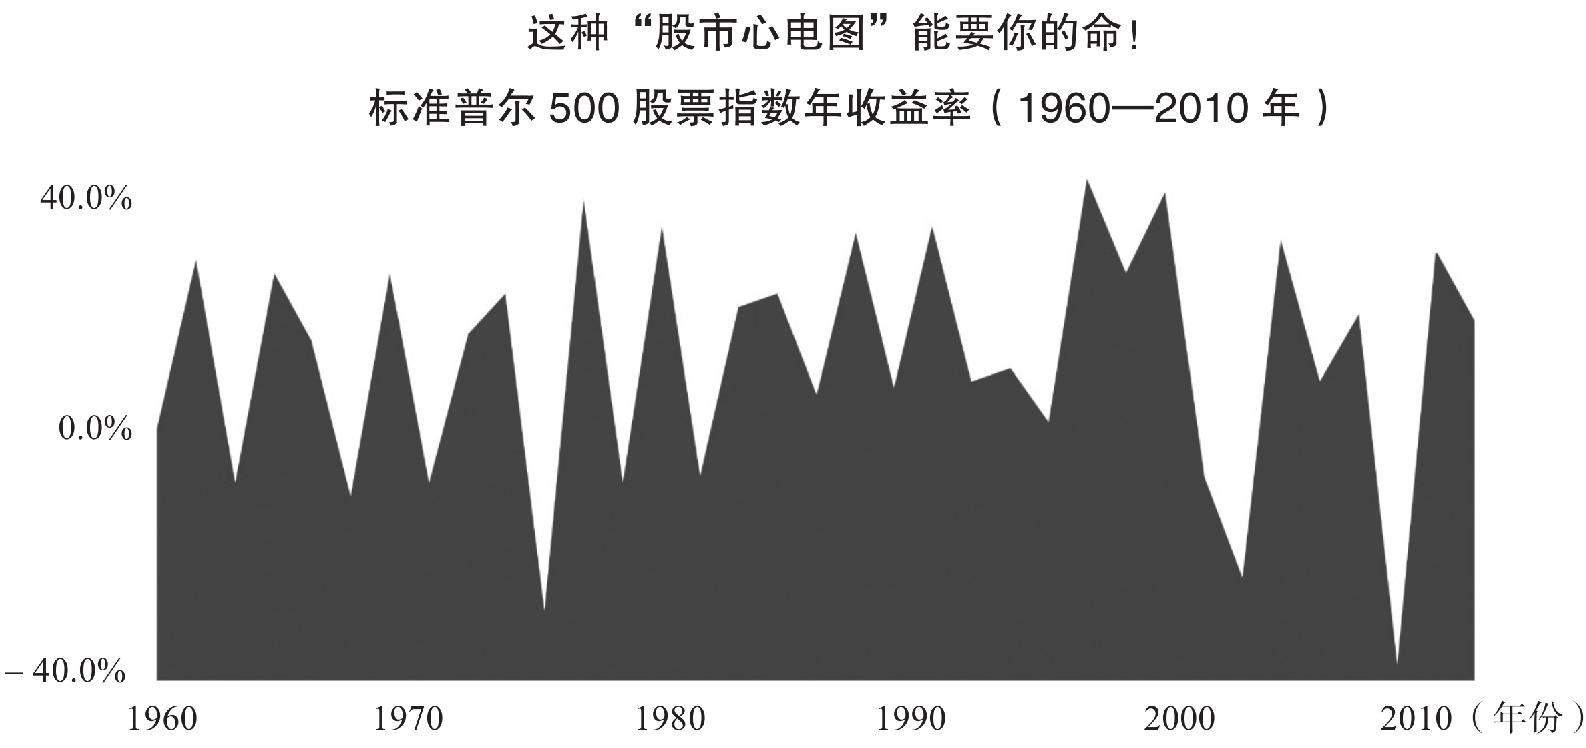
\includegraphics[width=0.92\linewidth,keepaspectratio]{image/13-1.jpg}
\caption{}\label{fig:13-1}
\end{figure}
